\documentclass[parskip=half, titlepage=firstiscover, captions=tableheading,bibliography=totoc,]{scrartcl}

%\usepackage{scrhack}

%\usepackage[utf8]{inputenc}

\usepackage{float}
\floatplacement{figure}{htbp}
\floatplacement{table}{htbp}

\usepackage{microtype}

\usepackage{booktabs}%alternativer Stil: alphabetic

\title{Optimale \LaTeX - Hilfe als Dokument}
\author{Carl Arne Thomann}

\date{\today} %Deutsches Datumsformat
\date{\textenglish\today} %Englisches Datumsformat

\usepackage{polyglossia}
\setmainlanguage{german}

\usepackage{biblatex}
\addbibresource{lit.bib}

\usepackage[autostyle]{csquotes}
\setotherlanguages{english}

\usepackage{blindtext}

\usepackage{amsmath}
\usepackage{amssymb}
\usepackage{mathtools}
%\usepackage{fontspec}
\usepackage[
	math-style=ISO,
	bold-style=ISO,
	sans-style=italic,
	nabla=upright,
	partial=upright,
]{unicode-math}

\usepackage{siunitx}

\usepackage{graphicx}
\usepackage{grffile}

\usepackage{mleftright} % ersetze im Code \left durch \mleft und \right durch \mright, sofern kein Space gewünscht wird bspw. bei Operatoren.

%\usepackage{placeins}
\usepackage[
font=normalsize,
labelfont=sc,
]{caption}
\usepackage{subcaption}

\usepackage{hyperref}
\usepackage{bookmark}

\usepackage{footmisc}

\usepackage{xfrac}

\usepackage{microtype}

%\usepackage{showframe}
%\usepackage{lua-visual-debug}

\DeclarePairedDelimiter{\bra}{\langle}{\rvert}
\DeclarePairedDelimiter{\ket}{\rvert}{\rangle}
\DeclarePairedDelimiterX{\braket}[2]{\langle}{\rangle}{#1 \delimsize\vert #2}

\usepackage{pdflscape}

\usepackage{expl3}
\usepackage{xparse}

\ExplSyntaxOn

\NewDocumentCommand \dif {m}
{
\mathinner{\mathup{d} #1}
}

\NewDocumentCommand \trollolo {m}
{
	Meine~Lieblingszahl~ist~\# #1
}

\let\vaccent=\v
\RenewDocumentCommand \v {}
{
	\TextOrMath{\vaccent}{\mathbf}
}

\ExplSyntaxOff

\usepackage{extdash} %anstelle von Bindestrichen "-", bitte "\-/" benutzen! Bei verbotenen Umbrüchen bitte \=/ benutzen, bspw. "$x$\=/Achse"

%
% Wichtige Reihenfolge: 
%	- amsmath bis unicode als solcher Block.
%	- extdash ganz zum Schluss
%	- scrhack ganz am Anfang nach \documentclass{}
%

\begin{document}
\maketitle
\section{Unicode-Zeichensatz}
Hallo Welt!
Umlaute wie öäü und andere deutsche Zeichen wie ß sind erlaubt und werden in \emph{vim} und \LaTeX erkannt.


\section{Listen}

\subsection{\emph{Liste}}

\subsection{\emph{Enumerate}}

\subsection{\emph{Description}}
\begin{description}
	\item[Sylvester Stallion] Lorem ipsum 
	\item[James ROFL] dolor sit
	\item[Edgar Thedt] amet
\end{description}


\section{Matheschriften mit \emph{amsmath} und \emph{unicode-math}}
\begin{table}
\begin{tabular}{llc}
	\backslash mathup		& aufrecht					& $\mathup{Beispiel}$ \\
	\backslash mathit		& kursiv					& $\mathit{Beispiel}$ \\
	\backslash mathsfup		& serifenlos, aufrecht		& $\mathsfup{Beispiel}$ \\
	\backslash 	mathsfit	& serifenlos, kursiv		& $\mathsfit{Beispiel}$ \\
	\backslash 	mathtt		& Schreibmaschine			& $\mathtt{Beispiel}$ \\
	\backslash 	mathbb		& Doppelschlag				& $\mathbb{Beispiel}$ \\
	\backslash 	mathbbit	& Doppelschrift, kursiv		& $\mathbbit{Beispiel}$ \\
	\backslash 	mathscr		& Skript					& $\mathscr{Beispiel}$ \\
	\backslash 	mathfrak	& Fraktur					& $\mathfrak{Beispiel}$ \\
	\backslash mathbfup		& fett, aufrecht			& $\mathbfup{Beispiel}$ \\
	\backslash mathbfit		& fett, kursiv				& $\mathbfit{Beispiel}$ \\
	\backslash 	mathbfsfup	& fett, serifenlos, aufrecht& $\mathbfsfup{Beispiel}$ \\
	\backslash 	mathbfsfit	& fett, serifenlos, kursiv	& $\mathbfsfit{Beispiel}$ \\
	\backslash 	matbfscr	& fett, Skript				& $\mathbfscr{Beispiel}$ \\
	\backslash 	mathbffrac	& fett, Fraktur				& $\mathbffrak{Beispiel}$ 
\end{tabular}
\end{table}

\section{Einheiten mit Fehler und Potenzen}

Die Angabe ist \SI{3.14}{\meter\per\second},
darin ist 
der Wert \num{3.14 +- 0.12}%\num{3.14+-0.12e12}
und
die Einheit \si{\meter\per\second}


\section{Figure und Subfigure}

\begin{figure}
	\centering
	
\includegraphics[width=\textwidth]{Pictures/peplogox.png}
	\caption{Das PeP-Logo.}
\end{figure}
\blindtext

\begin{figure}
\centering
\caption{Variationen an dem Logo von PeP et al. e.V.}
\begin{subfigure}{0.3\textwidth}
	
\includegraphics[width=\textwidth, angle=30]{Pictures/peplogox.png}
	\caption{mit einem Winkel von 30°}
\end{subfigure}
\hfill
\begin{subfigure}{0.3\textwidth}
	\centering
	
\includegraphics[width=\textwidth, height= 0.2cm]{Pictures/peplogox.png}
	\caption{auf \texorpdfstring{0,2 \, cm}{0,2cm} gequetscht.}
\end{subfigure}
\begin{subfigure}{0.3\textwidth}
	\centering
	
\includegraphics[width=\textwidth, angle= -30]{Pictures/peplogox.png}
	\caption{Das PeP-Logo.}
\end{subfigure}
\end{figure}

\section{\backslash texorpdfstring}
\backslash texorpdfstring\{ \LaTeX -Code \}\{ Unicode \}
muss benutzt werden, wenn \LaTeX -Code in Überschriften und an technischen Stellen, also jedenfalls nicht im Fließtext oder im Mathe-Modus.
In dieser Überschrift ist es ignoriert, um den Effekt zu sehen!

\section{Table}

\begin{table}
	\centering
	\caption{Eine Beispieltabelle mit verbotenen Vertikallinien}
	\label{tab}
	\begin{tabular}{c|ccc}
		\toprule
		1&2&3&4\\
		\midrule
		5&6&7&8\\
		5&6&7&8\\
		5&6&7&8\\
		5&6&7&8\\
		\bottomrule
	\end{tabular}
\end{table}

\begin{table}
	\centering
	\caption{Sortierung an Dezimalkommata}
	\label{tab2}
	\begin{tabular}{S[table-format=1.0] S[table-format=1.2] S[table-format=1.2] S[table-format=1.3]}
		\toprule
		\multicolumn{4}{c}{Willkürliche Werte}\\	
		\midrule
		5&2.21&7.21&3.321\\
		5&2.15&7.23&4.765\\
		5&2.39&7.43&2.134\\
		5&2.01&7.12&9.987\\
		\bottomrule
	\end{tabular}
\end{table}

\begin{table}
	\centering
	\caption{Sortierung an Dezimalkommata mit Messunsicherheiten\protect\footnotemark.}
	\label{tab3}
	\begin{tabular}{S[table-format=1.0] S[table-format=1.2] S[table-format=1.3] @{${}\pm{}$} S[table-format=0.3]}
		\toprule
		\multicolumn{4}{c}{Willkürliche Werte}\\	
		\midrule
		5&2.21&7.211&0.001\\
		5&2.15&7.232&0.005\\
		5&2.39&7.433&0.004\\
		5&2.01&7.124&0.007\\
		\bottomrule
	\end{tabular}
\end{table}
\footnotetext{syn. Fehler.

Es sind Fußnoten in Captions mit \backslash protect 
erlaubt, aber nicht erwünscht.}


\section{Bib\LaTeX}

Es exisieren die folgenden Bibliothekeintragsarten
\begin{description}
	\item[manual] Versuchsanleitungen: author, title, year
	\item[article] Standardartikel: author, title,year, journal, version, url, pages
	\item[inproceedings] Vorträge von Tagungen: author, booktitle, url, journal,pages, title, volume, year, version
	\item[online] Internetquellen: author, title, date, eprinttype, eprint
	\item[book]  Buch: author, title, date, publisher
\end{description}
\nocite{*}
\printbibliography


\section{Neue Befehle}
\trollolo{42}

Bra:$\bra{a}$ 
und Ket:$\ket{b}$
und Braket: $\braket{a}{b}$, 
aber nicht BraKet: $\bra{a}\ket{b}$ 
\begin{landscape}
	\begin{figure}[p]
	\centering
	
\includegraphics[width=\textwidth]{Pictures/peplogox.png}
	\caption{Das PeP-Logo.}
\end{figure}
\end{landscape}

\section{Plots der Ismo-Klasse: Zusammenspiel zwischen \texorpdfstring{\textsf{matplotlib}}{matplotlib} und \texorpdfstring{\LaTeX}{LaTeX} optimieren}
\begin{figure}[p]
	\centering
	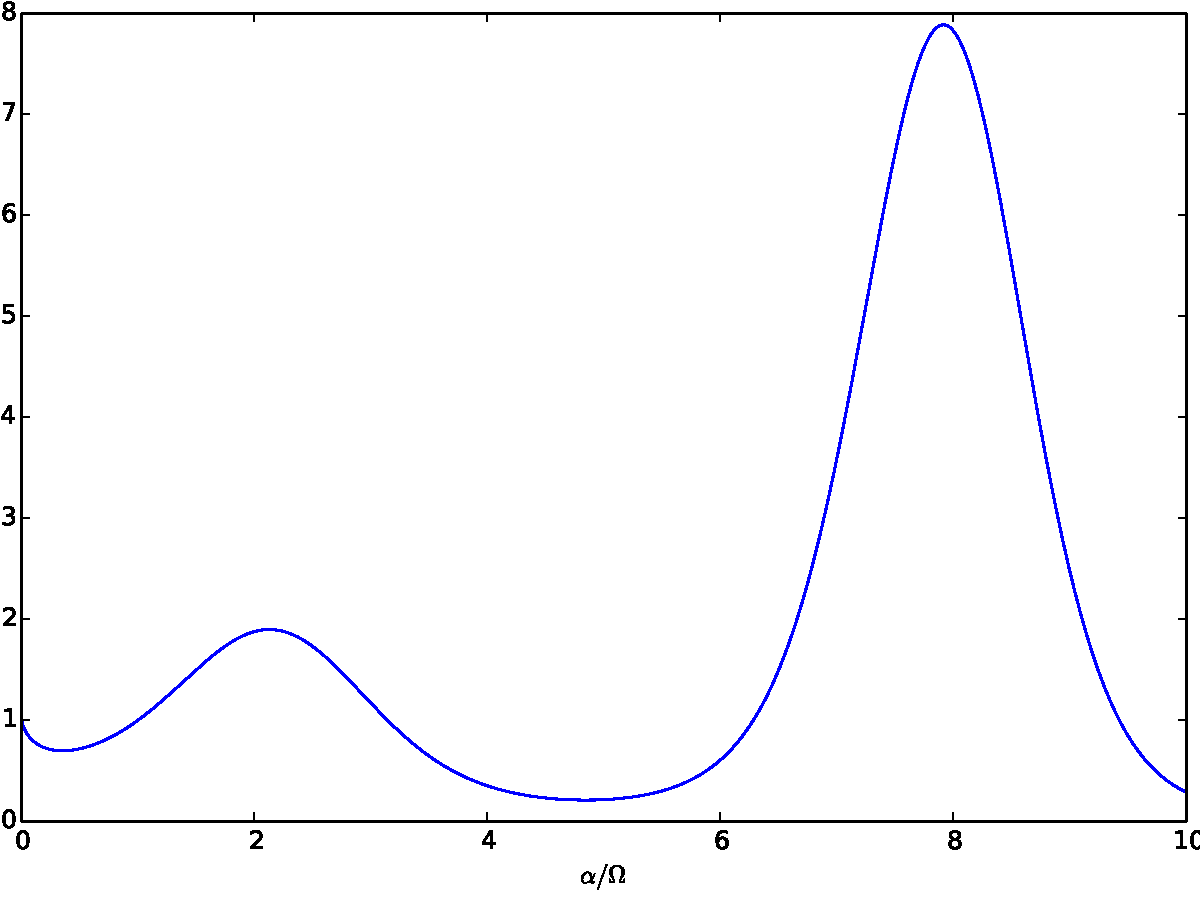
\includegraphics[width=0.9\textwidth]{Pictures/plot_schlecht.pdf}
	\caption{Standardplots}
\end{figure}
\begin{figure}[p]
	\centering
	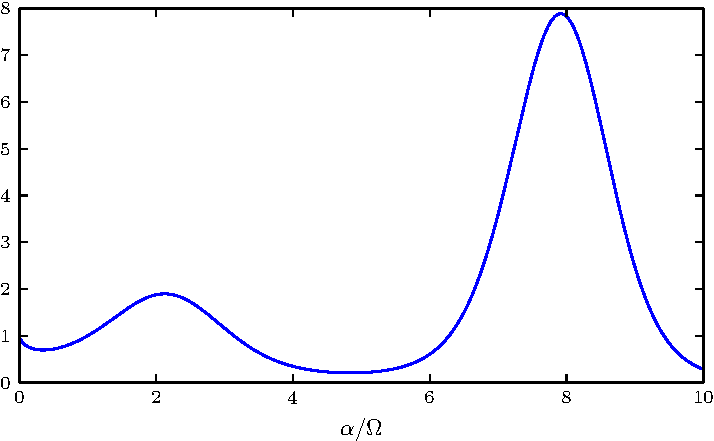
\includegraphics[width=0.9\textwidth]{Pictures/plot_gut.pdf}
	\caption{Ordentliche Plots}
\end{figure}

Die momentane Textweite ist \the\textwidth,
die Texthöhe ist \the\textheight.

Man beachte, dass die Standardgröße der \textsf{matplotlib}-Ausgabe gerade DIN A4 ist. 
Wird ein Plot von  Standardgröße auf \backslash \textsf{textwidth} gestaucht, so nimmt der Plot viel vertikalen Platz ein.
Mit der Konfigurationsdatei \emph{matplotlibrc} und der Erweiterung \emph{header-matplotlib.tex} kann einerseits ordentliches und uneingeschränktes \LaTeX, das schließt \backslash \textsf{si} aus \emph{siunitx} ein,  benutzt werden und
andererseits ein Ausgabeformat richtiger Größe vorgegeben werden.
Damit haben die Bezeichnungen an den Achsen die richtige, lesbare (!) Größe mit Serifen und der gesamte Plot eine über \textsf{plt.tight-layout} hinweg schlanke Form.

Um es genau zu nehmen, werden die schönsten Plotgrößen dadaurch erreicht, dass man mit dem Befehl \backslash\textsf{the}\backslash\textsf{textwidth} die momentane Weite anzeigen und dies als Maßgabe für die Plotweite nehmen kann.
Die formschönste Höhe dazu ist die des goldenen Schnittes, sodass die Plots ihr ursprüngliches DIN A4-Verhältnis beibehalten.

Inhalt der Konfigurationsdatei:
\textbf{\textsf{header-matplotlib.tex}}: \TeX in (r"\$ ... \$") erweitern\\
\backslash usepackage\{amsmath\} \\
\backslash usepackage\{amssymb\} \\
\backslash usepackage\{mathtools\} \\
\backslash usepackage\{fontspec\} \\
\backslash usepackage [\emph{hier Optionen, etwa ISO}] \{unicode-math\} \\
\backslash setmathfont\{Latin Modern Math\} \\
\backslash usepackage[per-mode-reciprocal,]\{siunitx\} \\

Inhalt der Konfigurationsdatei: 
\textbf{\textsf{matplotlibrc}}\\
backend : pgf \\
figure.figsize : 4.76, 2.94  \# Hier in Zoll die Maße eingeben\\
font.family : serif  \# Serifenschrift wirkt elegant \\
font.size : 11  \# Das ist die Standardschriftgröße in \LaTeX\\ 
legend.fontsize : medium \\
pgf.rcfonts : False \# Nicht weiter an Fonts pfuschen.\\
pgf.texsystem : lualatex \# TeX-Engine= LuaLaTeX\\
pgf.preamble : \backslash input\{header-matplotlib.tex\} \\
savefig.bbox : tight \\
savefig.pad\_inches : 0  \# Keinerlei weißen Rand lassen.\\
text.usetex : True \\
xtick.labelsize : 9 \\
ytick.labelsize : 9 \\

Eingabe im Terminal (nur) unter Linux: 
TEXINPUTS=\$(pwd): python script.py

\end{document}
